\documentclass[a4paper, draft]{article}
\pagestyle{headings}

\title{Machine learning and statistics}

\usepackage{amsmath,amsthm, amsfonts,amscd, amssymb, a4}
\usepackage[final]{graphicx}
\usepackage[final]{listings}
\usepackage{bbm}
\usepackage{empheq}
\usepackage{caption}

\renewcommand\lstlistingname{Algorithm}
\captionsetup[lstlisting]{singlelinecheck=false, margin=0pt, font={sf},labelsep=space,labelfont=bf}



% Numbering

%\numberwithin{section}{chapter}
%\numberwithin{equation}{chapter}

% Theorem environments

%% \theoremstyle{plain} %% This is the default
\newtheoremstyle{own}
    {3pt}                    % Space above
    {3pt}                    % Space below
    {\itshape}                   % Body font
    {}                           % Indent amount
    {\scshape}                   % Theorem head font
    {.}                          % Punctuation after theorem head
    {.5em}                       % Space after theorem head
    {}  % Theorem head spec (can be left empty, meaning ‘normal’)
    
\theoremstyle{own}
\newtheorem{thm}{Theorem}[section]
\newtheorem{cor}[thm]{Corollary}
\newtheorem{lem}[thm]{Lemma}
\newtheorem{prop}[thm]{Proposition}
\newtheorem{ax}{Axiom}[section]

%% \theoremstyle{definition}
\newtheorem{defn}{Definition}[section]

%% \theoremstyle{remark}
\newtheorem{rem}{Remark}[section]
\newtheorem*{notation}{Notation}
\newtheorem{algorithm}{Algorithm}[section]
\theoremstyle{remark}
\newtheorem{example}{Example}[section]

% Fix alignments

% \setlength{\parindent}{0cm}

\newcommand*\widefbox[1]{\fbox{\hspace{4em}#1\hspace{4em}}}
\newcommand*\fullbox[1]{\framebox[\columnwidth]{#1}}

%  Math definitions

% Fields
\newcommand{\R}{\mathbb{R}}
\newcommand{\C}{\mathbb{C}}
\newcommand{\Z}{\mathbb{Z}}
\newcommand{\Q}{\mathbb{Q}}
\newcommand{\N}{\mathbb{N}}
\newcommand{\quat}{\mathbb{H}}

%Groups 
\newcommand{\Lo}{\mathbf{O}(3,1)}
\newcommand{\SL}{\mathbf{SL}}
\newcommand{\SU}{\mathbf{SU}}
\newcommand{\Spin}{\mathbf{Spin}}
\newcommand{\Pin}{\mathbf{Pin}}
\newcommand{\SO}{\mathbf{SO}}
\newcommand{\Poincare}{\mathcal{P}}
\newcommand{\Poincarecov}{\widetilde{\mathcal{P}}}
\newcommand{\Poincareprop}{\widetilde{\mathcal{P}}_+^{\uparrow}}
\newcommand{\Aut}{\mathrm{Aut}}

% Rings
\newcommand{\End}{\mathrm{End}}
\newcommand{\CCl}{\mathbb{C}\mathrm{l}}
\newcommand{\Cl}{\mathrm{Cl}}
\newcommand{\Mat}{\mathrm{Mat}}

% Lie algebras

\newcommand{\spin}{\mathfrak{spin}}
\newcommand{\so}{\mathfrak{so}}
\newcommand{\su}{\mathfrak{su}}
\newcommand{\slc}{\mathfrak{sl}}

%Three-vectors
\newcommand{\xt}{\mathbf{x}}
\newcommand{\yt}{\mathbf{y}}
\newcommand{\pt}{\mathbf{p}}
\newcommand{\nt}{\mathbf{n}}
\newcommand{\sigmat}{\mathbf{\sigma}}

% Vector spaces
\newcommand{\Hil}{\mathcal{H}}

% Other
\newcommand{\calE}{\mathcal{E}}
\newcommand{\calD}{\mathcal{D}}
\newcommand{\calF}{\mathcal{F}}
\newcommand{\calP}{\mathcal{P}}
\newcommand{\Fock}{\mathcal{F}}
\newcommand{\Op}{\mathrm{Op}}

\DeclareMathOperator{\per}{per}
\DeclareMathOperator{\sign}{sgn}
\DeclareMathOperator{\logit}{logit}

\begin{document}
\maketitle


In these notes, we will take a closer look at a classical algorithm from the field of unsupervised learning - the expectation-maximization algorithm - and its applications to Gaussian mixture models. 

As a preparation, let us start with a very fundamental exercise - clustering. So suppose that we are given a data set which we suspect to consists of $K$ clusters. We want to identify these clusters, i.e. to each point in the dataset, we want to assign the number of the cluster to which the point belongs. 

More precisely, let us suppose that we are given a set ${\mathcal D} = \{ x_i, \dots, x_N\}$ of points in some $\R^d$ and a number $K$ of clusters. We want to identify the centre $\mu_i$ of each cluster and then assign the data points $x_i$ to some of the $\mu_j$, namely to the $\mu_j$ which is closest to $x_i$. We can encode the assignment of data points to clusters in a matrix $R_{ij}$ where $R_{ij} = 1$ if data point $x_i$ belongs to cluster $j$ with centre $\mu_j$. Thus each row of $R$ corresponds to a data point and is non-zero in exactly one column, where it is one. This is known as {\em 1-of-K encoding}.

For each value of $i$, the distance of $x_i$ to the centre of the cluster to which it is assigned is then given by
$$
\sum_j R_{ij} \| x_i - \mu_j |^2
$$
where we note that only one of the summands is different from zero. Assigning the data points to the clusters and positioning the centre points of the clusters then amounts to minimizing the loss function
$$
l(\mu, R) = \sum_i \sum_j R_{ij} \langle x_i - \mu_j , x_i - \mu_j \rangle
$$

Now let us see how we can optimize this function. For a fixed vector $\mu$ of cluster centres, we can easily minimize $R_{ij}$ by assigning each data point to the cluster whose centre is closest to $x_i$. Thus we set
$$
R_{ij} = 
\begin{cases}
1 & \text{if} \, j = \arg \min \| x_i - \mu_j |^2 \\
0 & \text{otherwise}
\end{cases}
$$
Conversely, given a matrix $R$ which we hold fixed, it is likewise easy to minimize $\mu_j$. As there are no further constraints on $\mu_j$, we can find the minimum by differentiating the loss function. We find that the derivative is zero if and only if
$$
0 = \sum_i R_{ij}(x_i - \mu_j)
$$
holds for all $j$. Assuming for a moment that each cluster has at least one data point assigned to it, i.e. that none of the columns of $R$ contains zeroes only, we can solve this by
$$
\mu_j = \frac{\sum_i x_i R_{ij}}{\sum_i R_{ij}}
$$
which is also easily seen to be a local minimum by taking the second derivative.

Note that this term has an obvious geometric interpretation. The denominator in this expression is the number of data points that are currently assigned to cluster $j$. The numerator is the sum of all data points assigned to this cluster. Thus the minimum is the mean of the positions of the data points that are currently assigned to the cluster (a physicist would call this the center of gravity of the cluster). This is the reason why this method is called the {\em k-means algorithm}. If no data points are assigned to the cluster, the loss function does not depend on $\mu_j$ and we can choose any value that we want. 

The algorithm now works as follows. First, we choose centres $\mu_j$ at will - it is common to use some of the data points for this purpose. Then we assign each data point to a centre using the formula for $R_{ij}$ derived above. We then adjust the centre points $\mu_j$ and reallocate the points to the new centres and so forth. 

From our discussion above, it is clear that each full iteration of this procedure will reduce the loss function. This does of course not imply that the algorithm converges to a global minimum, as it might get stuck in local minima or saddle points. In practice, the algorithm is executed until the cluster assignments and centres do not change any more substantially. 

\begin{figure}[ht]
\centering
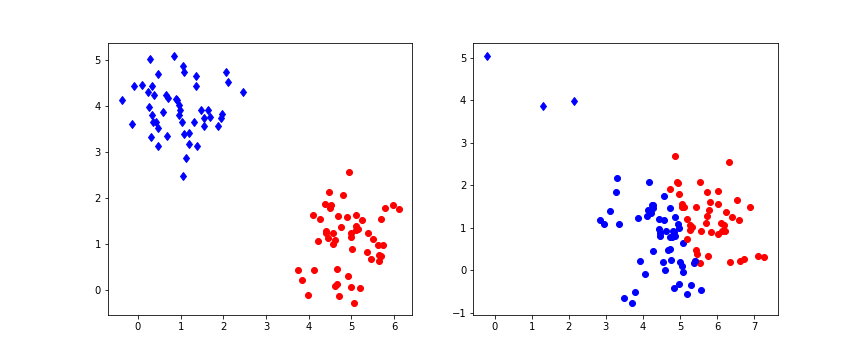
\includegraphics[width=1.0\linewidth]{KMeans}
\caption{K-means algorithm for two clusters}
\label{fig:KMeans}
\end{figure}

Diagram \ref{fig:KMeans} shows the result of applying this algorithm to a set of points that is organized in two clusters. To generate the data, 100 samples were drawn from 2-dimensional Gaussian distributions. On the left hand side, approximately half of the the samples were centered at the point $(5,1)$, the other samples at $(1,4)$, and both had standard deviation $0.6$. On the right hand side, the same centers were used, but only a small number of samples were drawn from the second distribution which had standard deviation $0.5$, whereas most samples came from the first distribution with standard deviation $0.8$. Then 10 iterations of the k-means algorithm were applied to the resulting sample set. The points in the sample were then plotted with a color indicating the assignment to clusters resulting from the matrix $R$. The actual cluster from which the sample was drawn is indicated by the shape - a point is cluster one, a diamond is cluster two.

We see that in the example on the left hand side, the algorithm has correctly assigned all points to their original cluster. For the example on the right hand side, the situation is different - the algorithm did actually assign significantly more points to the blue cluster, i.e. there are many wrong assignments (blue points). This does not change substantially if we increase the number of iterations, even with 100 iterations, we still see many wrong assigments for this example.

The K-means algorithm is very simple and straightforward, but seems to have limitations because it cannot determine the shape of a distribution, only its centre. It turns out that K-means is a special case of a broader class of algorithms that we now study, hoping to find more robust algorithms. In our example, we have generated sample data as a combination of two Gaussian distributions. Instead of just determining the assignment to a cluster and the means of the clusters, we could try to fit such a distribution to our data to derive additional information like the variance, to be able to sample and to apply Bayesian methods. Thus we try to fit our data to a model of the form
$$
P(x) = \sum_k \pi_k {\mathcal N}(x ; \mu_k, \Sigma_k)
$$
where ${\mathcal N}(x ; \mu_k, \Sigma_k)$ is a multivariate Gaussian distribution
with mean $\mu_k$ and covariance matrix $\Sigma_k$, i.e.
$$
{\mathcal N}(x ; \mu_k, \Sigma_k) = \frac{1}{\sqrt{(2\pi)^d \det(\Sigma)}}
\exp (-\frac{1}{2} \langle x - \mu_k, \Sigma_k^{-1}(x - \mu_k)\rangle)
$$
and the $\pi_k$ are non-negative real numbers with 
$$
\sum_k \pi_k = 1
$$
We can therefore interpret the coefficients $\pi_k$ as a probability measure $\pi(k) = \pi_k$ on $\{1, \dots, k\}$ and write the overall probability as a marginalization
$$
P(x) = \sum_k \pi(k) P(x | k) = \sum_k P(x,k)
$$
where 
$$
P(x , k) = {\mathcal N}(x ; \mu_k, \Sigma_k) \pi_k
$$
We interpret $\pi(k)$ as the probability to be in cluster $k$ and ${\mathcal N}(x ; \mu_k, \Sigma_k)$ as the probability distribution given the assignment to cluster $k$. In particular, we can sample from this distribution by first drawing a cluster $k$ with probability $\pi_k$ and then drawing $x$ from the distribution ${\mathcal N}(x ; \mu_k, \Sigma_k)$ (this approach to sampling by using conditional distributions is sometimes called {\em ancestral sampling}).

Let us now see how this equation looks like if we use a 1-of-K encoding or {\em one-hot} encoding. We introduce a random variable $Z$ that takes values in $\{ 0, 1\}^K$ with the additional constraint that only one of the $Z_k$ is allowed to be different from zero. We interpret $\pi_k$ as the probability 
$$
\pi_k = P(Z_k = 1)
$$
Then
$$
P(Z = z) = \prod_k \pi_k ^{z_k}
$$
and we can write
\begin{align}\label{eq:latentmodeljointdistribution}
P(X=x) = \sum_z P(Z=z) P(X=x | Z=z) = \sum_z P(x,z)
\end{align}
where $P(z)$ is as above and
$$
P(X = x | Z = z) = \prod_k {\mathcal N}(x ; \mu_k, \Sigma_k)^{z_k}
$$

We note that equation \ref{eq:latentmodeljointdistribution} is a very general type of distributions which reflects a common pattern in machine learning, namely the introduction of so called {\em latent variables}. In general, latent or hidden variables are random variables that are a part of the model which cannot be observed, i.e. are not part of the input or the output of the model. We have seen latent variables in action several times - adding hidden units to a neural network introduces latent variables and makes the model much more powerful, the hidden layer of a restricted Boltzmann machine serves as memory to learn features, and latent variables that are used to construct a mixture of Gaussians as above allow us to model a much broader class of distributions than a model with just one Gaussian. We will now investigate a general approach to apply the maximum likelihood method to models with latent variables which we will then apply to the special case of Gaussian mixtures wich is known as the {\em EM algorithm} and has been proposed in \cite{Dempster77}.

So let us now suppose that we are given some joint distribution of a random variable $X$ and and random variable $Z$ and are interested in maximizing the likelihood of an observed sample $x$ of the visible variable $X$. We also assume that the joint distribution depends on a parameter $\Theta$. Our aim is to maximize the log likelihood
$$
\ln P(x |\Theta) = \ln \sum_z P(x,z | \Theta)
$$
Even if the joint distribution belongs to some exponential family, the fact that we need to consider the logarithm of the sum and not the sum of the logarithms makes this expression and its gradient difficult to calculate. However, there is a different way to decompose the log likelihood. In fact, as
$$
P(z | x) = \frac{P(x,z)}{P(x)}
$$
we have
$$
\ln P(x | \Theta) = \ln P(x,z | \Theta) - \ln P(z | x,\Theta)
$$
Both terms in this expression can be interpreted as likelihoods. The first term is the {\em complete likelihood} of the observed value $x$ and the (hidden) value $z$, whereas the second one is the conditional likelihood of $z$ given $x$. Of course, the value of $z$ is not known. But this equation is still helpful - as the left hand side does not depend on $z$, we can take the average over all possible values of $z$ without changing the left hand side to obtain an expression that does not depend on $z$ any more. More precisely, let us assume that $q(z)$ is the probability mass function of any distribution over $z$. Then, as $\sum_z q(z) = 1$, we can write
\begin{align*}
\ln P(x | \Theta) &=  (\sum_z q(z)) \ln P(x | \Theta) \\ 
&= \sum_z q(z) \ln P(x,z | \Theta) - \sum_z q(z) \ln P(z | x, \Theta) \\
&= {\mathbbm E}_q \left[ \ln P(x,z | \Theta) \right] - 
{\mathbbm E}_q \left[  \ln P(z | x, \Theta)    \right]
\end{align*}
Let us now assume that we are given a value $\Theta$ of the parameter and let us try to understand how the likelihood changes if we pass from $\Theta$ to 
some $\Theta'$. To do this, let us specialize the above equation to the case that $q$ is the conditional distribution of $z$ given $\Theta$ and $x$. Then both terms turn into conditional expectations, and we have, for any choice of $\Theta'$,
$$
\ln P(x | \Theta') = 
{\mathbbm E} \left[  \ln P(x,z | \Theta')  | x, \Theta   \right]
-
{\mathbbm E} \left[  \ln P(z | x,\Theta') | x, \Theta      \right]
$$
Let us now introduce the notation
$$
Q(\Theta'; \Theta) = {\mathbbm E} \left[  \ln P(x,z | \Theta')  | x, \Theta \right]
$$
For a given value $\Theta$, this is a function of $\Theta'$. The EM-algorithm is now based on the observation that in order to maximize $\ln P(x | \Theta')$, we can maximize this function which is often easier to work with.
\begin{thm}[\cite{Dempster77}]\label{thm:em}
Suppose that $X$ is some random variable and that $Z$ is a finite random variable, so that the joint distribution of $X$ and $Z$ is determined by some parameter $\Theta$. Suppose that we are given some value $\Theta$ of this parameter and a sample $x$ of $X$ and define a function $Q$ by
$$
Q(\Theta'; \Theta) = {\mathbbm E} \left[  \ln P(x,z | \Theta')  | x, \Theta \right]
$$
Then, for any $\Theta'$, we have that
$$
\ln P(x | \Theta') - \ln P(x | \Theta) \geq
Q(\Theta' ; \Theta) - Q(\Theta ; \Theta) 
$$
with equality if and only if 
$$
P(z | x, \Theta') = P(z | x, \Theta)
$$
for all $z$.
\end{thm}

\begin{proof}
For any value of $\Theta'$, we have
$$
\ln P(x | \Theta') - \ln Px | \Theta) = 
Q(\Theta' ; \Theta) - Q(\Theta ; \Theta) 
+
\sum_z P(z | x, \Theta) \ln \frac{P(z | x, \Theta)}{P(z | x, \Theta')}
$$
Now the term on the right hand side is nothing but the Kullback-Leibler divergence
between the conditional distributions of $z$ given $x$ and $\Theta'$ respectively
$\Theta$. However, it is well known that the Kullback-Leibler divergence is always non-negative and is zero if and only if the two distributions coincide. This proves our assertions.
\end{proof}

\begin{cor}\label{cor:emalgorithm}
Suppose that $\Theta^{(t)}$ is a sequence of parameters for a latent variable model as described in theorem \ref{thm:em}. If
$$
Q(\Theta^{(t+1)};\Theta^{(t)} \geq Q(\Theta^{(t)}) ; \Theta^{(t)})
$$
for all $t$, then
$$
\ln P(x, \Theta^{(t+1)}) \geq \ln P(x, \Theta^{(t)})
$$
for all $t$ with equality if and only if
$$
Q(\Theta^{(t+1)};\Theta^{(t)} = Q(\Theta^{(t)}) ; \Theta^{(t)})
$$
and
$$
P(z | x, \Theta^{(t+1)}) = P(z | x, \Theta^{(t)})
$$
for all z. In other words, a sequence of parameters for which $Q$ is non-decreasing will delivery a sequence of parameters for which the log-likelihood is non-decreasing.
\end{cor}

This result now suggests the following  {\em EM algorithm} for maximizing the likelihood of a given set of observations. Suppose we are given some value $\Theta^{(t)}$ for the variables. We then calculate the expectation value
$$
Q(\Theta ; \Theta^{(t)}) = \sum_z  P(z | x, \Theta^{(t)}) \ln P(x,z | \Theta)  
$$
and express this as a function of $\Theta$. This step is called the {\em expectation step} of the algorithm. We then choose $\Theta^{(t+1)}$ so that it maximizes $Q$, i.e.
$$
\Theta^{(t+1)} =  \arg \max Q(\cdot ; \Theta^{(t)})
$$
This step is called the {\em maximization step}. We then repeat this procedure with $\Theta^{(t+1)}$ in place of $\Theta^{(t)}$ and so forth. The corollary above will then guarantee that the log likelihood is non-decreasing with every step of the algorithm. Of course, this does not imply that the sequence $\Theta^{(t)}$ converges nor does it imply that we reach a global maximum. Some additional conditions are needed for this, and we refer the reader to \cite{Dempster77} and \cite{RobertCasella1999} for some examples for conditions that guarantee convergence. In practice, the algorithm is usually applied until the change of the likelihood drops below a certain threshold or until a certain number of iterations has been completed.

	As an example where the EM algorithm turns out to be useful, let us return to the problem of a mixture of Gaussians and let us try to derive an expression for $Q$. Here the parameter $\Theta$ is given by 
	$$
	\Theta = (\mu, \pi, \Sigma)
	$$
	We consider a random variable $X$ which has $N$ components, each of which being a vector $X_n$ in a $d$-dimensional space. Similarly, $Z$ consists of $N$ components $z_n$ which again are subject to the restriction that only one of the $z_{nk}$ be different from zero. We assume that the joint representation of our model is given by
	$$
	P(x , z) = \prod_n \prod_k \pi_k^{z_{nk}}{\mathcal N} (x_n, \mu_k , \Sigma_k)^{z_{nk}}
	$$
from which we immediately obtain by integrating over all $x_n$ and applying Fubinis theorem that
$$
P(z) = \prod_n \prod_k \pi_k^{z_{nk}} = \prod_n P(z_n)
$$ and consequently that
the conditional probability of $X$ given $Z$ 
is 
$$
P(X = x | Z = z) = \prod_n \prod_k {\mathcal N} (x_n, \mu_k , \Sigma_k)^{z_{nk}}
$$

Let us first calculate the conditional probabilities of $z$. Using Bayes theorem, we can write
\begin{align*}
P(Z = z | X = x) &= \frac{1}{P(X)} P(X=x | Z=x) P(Z = z)    \\
&= \frac{1}{P(X)} \prod_n \prod_k {\mathcal N}(x_n ; \mu_k, \Sigma_k)^{z_{nk}} \pi_k^{z_{nk}}
\end{align*}
As this factors over $n$, we can conclude that the $Z_n$ are independent given $X$. and that the conditional probability of one component $Z_n$ is given by
$$
P(Z_n = z_n | X = x) = \frac{1}{P(X_n = x_n)} \prod_k {\mathcal N}(x_n ; \mu_k, \Sigma_k)^{z_{nk}}
$$
This allows us to calculate the conditional expectation of $Z_{nk}$ for a given pair of indices $n,k$. We find that
\begin{align*}
{\mathbbm E}(Z_{nk} | x,\Theta ) = P(Z_{nk} = 1 | x, \Theta) = \frac{\pi_k {\mathcal N}(x_n ; \mu_k, \Sigma_k)}
{\sum_{j} \pi_j {\mathcal N}(x_n ; \mu_j, \Sigma_j) }
\end{align*}
This quantity is called the {\em responsibility} $r_{nk}$ of the cluster $k$ for the data point $x_n$ and measures how likely it is that the data points belongs to the cluster $k$. Note that each responsibility is a function of $\Theta$, so that to be precise, we would have to write
$$
r_{nk} = r_{nk}(\Theta)
$$
A short calculation using the fact that for each $z_n$, only one of the coordinates is different from zero, now shows that we can express $Q$ as follows.
$$
Q(\Theta'; \Theta) = \sum_n
\sum_k r_{nk} \ln \pi'_k 
+ \sum_n \sum_k r_{nk} \ln {\mathcal N}(x ; \mu'_k, \Sigma'_k)
$$
where the responsibilities are calculated using $\Theta$. This looks tractable - the first term  only depends on $\pi'$, whereas the second term only depends on $\mu'$ and $\Sigma'$. We can therefore maximize all components independently. We start with the second term. A short calculation shows that the gradient with respect to $\mu$ is given by
$$
\nabla_\mu \ln {\mathcal N}(x; \mu , \Sigma) = \Sigma^{-1}(x-\mu)
$$
so that the maximum with respect to $\mu_k$ is given by the condition
$$
\sum_n r_{nk} \Sigma_k^{-1} (x_n - \mu'_k) = 0
$$
This is equivalent to
$$
\sum_n r_{nk} (x_n - \mu'_k) = 0
$$
so that we obtain 
\begin{align}\label{eq:maxlikelihoodmixturecentres}
\mu'_k = \frac{\sum_n r_{nk} x_n}{\sum_n r_{nk}}
\end{align}
This starts to look familiar - this is the same expression that we did obtain for the cluster centers for the k-means algorithm! In fact, if we arrange the $r_{nk}$ as a matrix, the denominator is the sum across column $k$ and the numerators is the weighted sum over all data points. However, there is one important difference - it is no longer true that given $n$, only one of the $r_{nk}$ will be different from one. Instead, the $r_{nk}$ are {\em soft assignments} that model the probability that the data point $x_n$ belongs to cluster $k$. 

No let us consider the derivatives with respect to $\Sigma_k$. This is a bit more complicated, and to organize the calculations, we need the following 

\begin{lem}
Suppose that $A$ is an invertible matrix. Then for each pair of indices $i,j$, we have
$$
\frac{\partial }{\partial A_{ij}} \ln \det A = (A^{-1})_{ji}
$$
\end{lem}

\begin{proof}
Let $\tilde{A}$ be the matrix whose element at row $l$ and column $m$ is given by 
$(-1)^{l+m}$ times the determinant of the submatrix obtained from $A$ by removing column $l$ and row $m$ (this is known as the {\em adjugate matrix}). 
Now the Laplace formula for the determinant
$$
(\det A) {\mathbbm 1} = A \tilde{A}
$$
tells us that
$$
\det A = \sum_k A_{ik} \tilde{A}_{ki}
$$
so that
$$
\frac{\partial }{\partial A_{ij}} \det A = 
\sum_k \frac{\partial }{\partial A_{ij}} A_{ik} \tilde{A}_{ki}
$$
Now the number $\tilde{A}_{ki}$ is obtained from $A$ by removing row $i$ and column $k$, in particular it does not depend on $A_{ij}$ because that element is located in the row that is removed. Hence
$$
\frac{\partial }{\partial A_{ij}} \tilde{A}_{ki} = 0
$$
and we find that
$$
\frac{\partial }{\partial A_{ij}} \det A  = \tilde{A}_{ji}
$$
which, using the Laplace formula once more, gives
$$
\frac{\partial }{\partial A_{ij}} \det A = (\det A) A^{-1}_{ji}
$$
Therefore
$$
\frac{\partial }{\partial A_{ij}} \ln \det A = \frac{1}{\det A} \frac{\partial }{\partial A_{ij}} \det A = A^{-1}_{ji}
$$
as claimed.
\end{proof}

Let us now use this result from linear algebra to determine the derivative of $Q$ with respect to the covariance matrix. Recall that
$$
{\mathcal N}(x ; \mu, \Sigma) = \frac{1}{\sqrt{(2\pi)^d \det(\Sigma)}}
\exp (-\frac{1}{2} \langle x - \mu, \Sigma^{-1}(x - \mu)\rangle)
$$
It is easier to express the minimum in terms of the coefficients of the inverse matrix $S = \Sigma^{-1}$. The derivative of the logarithm of this term with respect to $\Sigma^{-1}$ is given by
\begin{align*}
\frac{\partial}{\partial S_{ij}} \ln  {\mathcal N}(x ; \mu, \Sigma) 
& = \frac{1}{2} \frac{\partial}{\partial S_{ij}} \ln \det S
 - \frac{1}{2} \frac{\partial}{\partial S_{ij}} \langle x - \mu, S(x - \mu)\rangle) \\
&=  \frac{1}{2} \left[ 
\Sigma_{ji} 
-
(x - \mu)_i(x - \mu)_j
\right]
\end{align*}
which, in a short hand matrix notation, can be written as
$$
\frac{\partial}{\partial \Sigma^{-1}} \ln  {\mathcal N}(x ; \mu, \Sigma) 
= \frac{1}{2} \left[ 
\Sigma^T 
-
(x - \mu)(x - \mu)^T
\right]
$$
where we interpret $x - \mu$ as a column vector. 
Let us now apply this to $Q$. We find that
$$
\frac{\partial}{\partial \Sigma'^{-1}_k} Q 
= \frac{1}{2}
\sum_n  r_{nk}
\left[
\Sigma_k^T 
-
(x_n - \mu_k)(x_n - \mu_k)^T
\right] 
$$
Setting this to zero, we obtain the condition
$$
\sum_n  r_{nk} \Sigma_k^T = \sum_n  r_{nk} (x_n - \mu_k)(x_n - \mu_k)^T
$$
Let us now set
$$
N_k = \sum_n r_{nk}
$$
which can be interpreted as the number of soft assignments of points to cluster $k$. Then the left hand side of this equality is simply $N_k \Sigma_k^T$, and we obtain the solution
$$
\Sigma'_k = \frac{1}{N_k} \sum_n r_{nk} (x_n - \mu_k)(x_n - \mu_k)^T
$$
Note that this gives us a symmetric matrix, which justifies our approach (by setting the gradient to zero, we have located an extremum in the space of all matrices, which now turns out to be again in the subspace of symmetric matrices). 

When applying this in combination with the maximization with respect to the $\mu_k$, we need to apply the new values $\mu'_k$ first (which do not depend on $\Sigma$), so that we should rather choose
\begin{align}\label{eq:maxlikelihoodmixturesigma}
\Sigma'_k = \frac{1}{N_k} \sum_n r_{nk} (x_n - {\mu'}_k)(x_n - {\mu'}_k)^T
\end{align}
Finally, let us turn to maximizing the term
$$
\sum_n
\sum_k r_{nk} \ln \pi'_k = \sum_k N_k \ln \pi'_k
$$
Here, we need to maximize subject to the constraint that
$$
1 = \sum_k \pi'_k 
$$
To do this, we introduce a Lagrange multiplier $\lambda$. Thus we need to maximize the function
$$
\sum_k N_k \ln \pi'_k + \lambda (1 - \sum_k \pi'_k )
$$
Taking partial derivatives, we find that the gradient of this function vanishes if 
$$
\frac{N_k}{\pi'_k} = \lambda
$$
for all $k$, i.e. if
$$
N_k = \lambda \pi'_k
$$
for all $k$. 
Summing over all $k$ and observing that the sum across the rows of the matrix $R$ is always one, so that 
$$
\sum_k N_k = N
$$
we find that
$$
N = \lambda \sum_k \pi'_k = \lambda
$$
so that our solution will be
\begin{align}\label{eq:maxlikelihoodmixturepi}
\pi'_k = \frac{N_k}{N}
\end{align}
Again, this is intuitively very appealing - the probability to be in cluster $k$ is updated to be the number of points with a soft assignment to $k$ divided by the total number of assignments.

Having completed these rather lengthy calculations, we are now able to combine corollary \ref{cor:emalgorithm} and the equations \eqref{eq:maxlikelihoodmixturecentres}, \eqref{eq:maxlikelihoodmixturepi} and \eqref{eq:maxlikelihoodmixturesigma} into the {\em EM algorithm for Gaussian mixtures} (see algorithm \ref{lst:emgaussianmixture})


\begin{lstlisting}[mathescape=true,frame=single, label=lst:emgaussianmixture, float=ht,
captionpos=t, caption=EM algorithm for Gaussian mixture]
Assign starting values to $\Sigma_k$, $\mu_k$ and $\pi_k$ 
For each iteration do
  Calculate the responsibility matrix 
  
    $R_{nk} = \pi_k {\mathcal N}(x_n ; \mu_k, \Sigma_k) \big/ \sum_j \pi_j {\mathcal N}(x_n ; \mu_j, \Sigma_j)$
  
  Let 
    $N_k = \sum_n R_{nk}$ 
  Let 
    $\mu_k = (\sum_n R_{nk} x_n) / N_k$
  Let 
    $\Sigma_k = (\sum_n R_{nk} (x_n - \mu_k)(x_n - \mu_k)^T) / N_k$
  Let 
    $\pi_k = N_k / N$  
Done 
\end{lstlisting}

Let us see how this algorithm performs in practice. Diagram \ref{fig:GMM} shows two samples that have been generated as a mixture of two Gaussians. In the row at the top, we have applied 100 iterations of the k-Means algorithm. We see that the k-Means algorithm is not able to separate the two clusters, there is a large number of blue dots which have been sampled from the first mixture component, but are assigned incorrectly to the second component.

In contrast to this, the lower row shows the result of applying 100 iterations of the EM algorithm to the two samples. For both samples, the EM algorithm yields the expected result and is able to correctly separate the points.

\begin{figure}[ht]
	\centering
	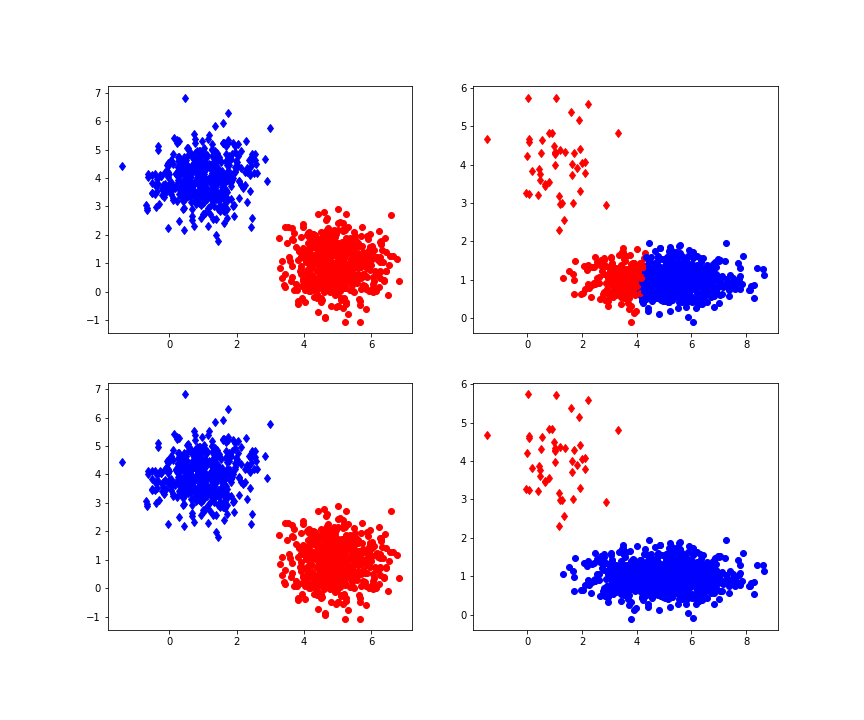
\includegraphics[width=1.0\linewidth]{GMM}
	\caption{EM algorithm for Gaussian mixtures}
	\label{fig:GMM}
\end{figure}

To be able to handle larger data sets efficiently, a vectorized implementation in Python is extremely helpful, which avoids loops and sums over the number of sample points (loops over the number of clusters are more difficult to avoid but less problematic because that number tends to be small). The expectation step can 
be realized with a few lines of code, a possible implementation is shown 
in listing \ref{lst:estepPython}.

\begin{lstlisting}[frame=single,language=Python,label=lst:estepPython, caption=Expectation step in Python]
R = np.zeros(shape=(N,K))
for k in range(K):
	R[:,k] = weights[k]*multivariate_normal(
	                        means[k],cov[k]).pdf(S)
R = (R.T / np.sum(R, axis=1)).T
\end{lstlisting}

Here we assume that the covariance matrices $\Sigma_k$ are stored in a list \verb+cov+ of which each elements is a $d \times d$ matrix, where $d$ is the dimension of the feature vectors, and that the sample vectors are stored in a matrix \verb|+|S+ with dimension
$N \times d$. The vectors \verb|+|weights+ contains the weights $\pi_k$, and we use the 
\verb+multivariate_normal+ class from the package \verb+scipy.stats+ to calculate the probability density function of the Gaussian.

The maximization step can also be mostly implemented in terms of matrix operations and is shown in listing \ref{lst:mstepPython}. 

\begin{lstlisting}[frame=single,language=Python,label=lst:mstepPython, caption=Maximization step in Python,float=ht]
#
# Calculate N_k and means 
#
Nk = np.sum(R, axis=0)    
means = np.dot(R.T, S)
means = (means.T / Nk).T

#
# Calculate covariance matrix
#
cov = []        
for k in range(K):
    y = S[:,:] - means[k,:]
    outer = np.multiply.outer(y,y)
    O = np.diagonal(np.swapaxes(outer,1,2)).T
    _cov = np.dot(R[:,k], np.swapaxes(O, 0,1)) / Nk[k]
    cov.append(_cov)
# 
# now update weights
#
weights = Nk / N
\end{lstlisting}

To compute the covariance matrix $\Sigma_k$, we first build a matrix \verb|O| such that \verb|O[n,:,:]| is the outer product of $x_n - \mu_k$ with itself. We can then use
the \verb|np.dot| operation to express the sum over $n$. This avoids an inner loop over $n$ and speeds up the computation significantly.

Note that the EM algorithm can also be applied to classification problems. In fact, once we have determined the parameters, we can easily compute the conditional probabilities $P(Z | X)$ for any new data point $X$ - this will simply be given by the formula for the responsibilities. As an example, let us again consider the Iris data set. Here we have four features, i.e. a four-dimensional data set, that we try to organize in three cluster.

Table \ref{table:irisdataem} lists the result of applying the EM algorithm with 200 iterations to the Iris data set.

\begin{table}[ht]
	\centering
	\begin{tabular}{|c|c|c|c|}
	\hline 
	Cluster & Iris setosa & Iris versicolor & Iris virginica \\
	\hline
	1 & 0 & 45 & 0 \\
	2 & 50 & 0 & 0 \\
	3 & 0 & 5 & 50 \\
	\hline
	\end{tabular}
	\caption{Classifying the Iris data set with the EM algorithm}
	\label{table:irisdataem}
\end{table}

Each column lists the number of flowers from each of the three species that were assigned to cluster 1,2 and 3. We see that all samples from the first and third species are assigned to the clusters 2 und 3. For the second species, 5 data points are incorrectly assigned to cluster 3, whereas all the other points are assigned to cluster 1. Thus 5 out of 150 sample points were misclassified, an error rate which is in the same range as the error rate for the multinomial regression model studied earlier. The final value of the loss function for this clustering was $\approx 181$.

It should be noted that the error rate depends heavily on the initial assignment of the cluster centres. If random assignments are used, then several runs were required to achieve this low error rate, whereas other runs resulted in error rates of up to 30 \%. In these cases, the algorithm got trapped in local minima, with a loss function of $\approx 200$.

Again, it is instructive to compare the performance with the k-means algorithm. I have conducted several runs with a k-means algorithm with 200 iterations, but in none of these runs, the number of errors dropped below 16. So again, the EM algorithm turns out to deliver better results than the plain k-means algorithm, but it requires several trials with random initial values for the cluster centres to locate the (apparently) global minimum. 

Finally, we remark that for other models, the E-step might be much more difficult and Monte Carlo techniques can be employed to approximate the expectation values - we refer the reader to \cite{RobertCasella1999} section 5.4 for a short discussion of the Monte Carlo EM algorithm.




%%%%%%%%%%%%%%%%%%%%%%%%%%%%%%%%%%%%%%%%%%%%%%
%% Bibliography
%%%%%%%%%%%%%%%%%%%%%%%%%%%%%%%%%%%%%%%%%%%%%%

\begin{thebibliography}{9}
	
\bibitem{Bauer}
H.~Bauer,
{\em Wahrscheinlichkeitstheorie},
de Gruyter, Berlin, New York 1991
	

\bibitem{Bishop}
C.M.~Bishop, 
{\em Pattern recognition and machine learning},
Springer, New York 2006

\bibitem{Klenke}
A.~Klenke,
{\em Probability theory}
Springer, London 2008

\bibitem{MehtaSchwab}
P.~Mehta,D.J.~Schwab, 
{\em An exact mapping between the Variational Renormalization Group and Deep Learning},
arXiv:1410.3831, 2014

\bibitem{Cox}
D.R.~Cox,
{\em The regression analysis of binary sequences},
Journal of the Royal Statistical Society, Series B, Vol. 20, No. 2 (1958), pp 215--242

\bibitem{Shannon}
C.E.~Shannon,
{\em A mathematical theory of communication}, 
The Bell System Technical Journal {\em Vol. 27}, pp. 379--423, pp. 623--656, July, October 1948


\bibitem{CasellaBerger}
G.~Casella, R.L.~Berger,
{\em Statistical inference},
Duxbury Press 2002

\bibitem{Schervish}
M.J.~Schervish,
{\em Random number generation and Monte Carlo Methods},
Springer Verlag, New York, Berlin, Heidelberg 2003

\bibitem{LehmannRomano}
E.L.~Lehmann, J.P.~Romano,
{\em Testing statistical hypothesis},
Springer, New York 2005

\bibitem{Theano}
The Theano development team
{\em Theano: A Python framework for fast computation of mathematical expressions},
arXiv:1605.02688

\bibitem{Tensorflow}
M.~Abadi et.al.,
{\em TensorFlow: Large-Scale Machine Learning on Heterogeneous Distributed System},
arXiv:1603.04467

\bibitem{RHW}
D.E.~Rumelhart, G.E.~Hinton, R.J.~Williams,
{\em Learning internal representations by error propagation}, in
{\em Parallel distributed processing}, edited by D.E.~McClelland and J.L.~Rumelhart, MIT Press, 1986

\bibitem{MeynTweedie}
S.P.~Meyn, R.L.~Tweedie,
{\em Markov chains and stochastic stability},
Cambridge University Press, 2008

\bibitem{MCMCHandbook}
S.~Brooks, A.~Gelman, C.L.~Jones,X.L.~Meng (ed.)
{\em Handbook of Markov chain Monte Carlo},
Chapman \& Hall / CRC Press, Boca Raton 2011

\bibitem{RobertsTweedie1996}
G.O.~Roberts, R.L.~Tweedie,
{\em Geometric Convergence and Central Limit Theorems for Multidimensional Hastings and
	Metropolis Algorithms},
Biometrika, Vol. 83, No. 1 (1996), pp. 95--110

\bibitem{Tierney1994}
L.~Tierney, 
{\em Markov chains for exploring posterior distributions},
Ann. Stat. Vol. 22, No. 4 (1994), pp. 1701--1728

\bibitem{RobertCasella1999}
C.P.~Robert, G.~Casella,
{\em Monte Carlo Statistical Methods},
Springer, New York 1999


\bibitem{Hastings1970}
W.K.~Hastings,
{\em Monte Carlo sampling methods using Markov chains and their applications},
Biometrika, Vol. 57 No. 1 (1970), pp. 97--109


\bibitem{Peskun1973}
P.H.~Peskun,
{\em Optimum Monte-Carlo sampling using Markov chains},
Bio\-metrika, Vol. 60, No. 3 (1973), pp. 607--612

\bibitem{RobertsRosenthal2006}
G.O.~Roberts, J.S.~Rosenthal,
{\em Harris recurrence of Metropolis-within-Gibbs and transdimensional Markov chains},
Ann. Applied. Prob., Vol. 16, No. 4 (2006), pp. 2123--2139

\bibitem{KemenySnell}
J.G.~Kemeny, J.L.~Snell,
{\em Finite Markov chains},
Springer Verlag, New York, Berlin, Heidelberg, Tokyo 1976

\bibitem{Revuz}
D.~Revuz,
{\em Markov chains},
North Holland, Amsterdam, New York, Oxford 1984


\bibitem{Rudin}
W.~Rudin,
{\em Real and complex analysis},
McGraw Hill, London, New York 1970

\bibitem{Metropolis1953}
N.~Metropolis,A.W.~Rosenbluth, M.N.~Rosenbluth, A.H.~Teller, E.~Teller,
{\em Equation of state calculation by fast computing machines},
J. Chem. Phys. Vol. 21, No. 6 (1953), pp. 1087--1092

\bibitem{ChanGeyer1994}
S.~Chan, C.T.~Geyer,
{\em Discussion: Markov chains for exploring posterior distributions},
Ann. Stat. Vol. 22, No. 4 (1994), pp. 1747--1758


\bibitem{Neal1993}
R.M.~Neal, 
{\em Probabilist inference using Markov chain Monte Carlo methods}, 
Technical Report CRG-TR-93-1, Department of Computer Science, University of Toronto, 1993

\bibitem{Neal1996}
R.M.~Neal,
{\em Bayesian Learning for neural networks},
Springer, New York 1996


\bibitem{Callen}
H.B.~Callen,
{\em Thermodynamics and an introduction to Thermostatistics},
Wiley, New York 1985

\bibitem{Hopfield1982}
J.J.~Hopfield,
{\em Neural networks and physical systems with emergent collective computational
	abilities},
Proc. Nat. Acad. Sci. Vol. 79, No. 8 (1982), pp. 2554--2558

\bibitem{Schroeder}
D.V.~Schroeder,
{\em An introduction to thermal physics},
Addison-Wesley, San Francisco 2000

\bibitem{Hebb}
D.O.~Hebb,
{\em The organization of behaviour},
Wiley, New York 1949

\bibitem{Bengio2009}
Y.~Bengio,
{\em Learning deep architectures for AI},
Foundations and Trends in Machine Learning Vol. 2, No. 1 (2009), 1--127

\bibitem{MacKay}
D.~MacKay,
{\em Information Theory, Inference and Learning Algorithms},
Cambridge University Press, Cambridge 2003

\bibitem{Ising1924}
E.~Ising,
{\em Beitrag zur Theorie des Ferromagnetismus},
Zeitschrift f. Physik, Vol. 31, No.1 (1924), 253--258

\bibitem{Hinton2002}
G.~Hinton,
{\em Training products of experts by minimizing contrastive divergence},
Journal Neural Computation Vol. 14, No. 8 (2002), 1771--1800

\bibitem{FischerIgel2014}
A.~Fischer, C.~Igel,
{\em Training restricted Boltzmann machines: an introduction},
Pattern Recognition Vol. 47 (2014), pp 25--39

\bibitem{Hinton2010}
G.~Hinton,
{\em A practical guide to training restricted Boltzmann machines},
Technical Report University of Montreal TR-2010-003

\bibitem{BengioRoux2007}
N.~Le Roux, Y.~Bengio,
{\em Representational Power of Restriced Boltzmann machines and Deep Belief Networks},
Journal Neural Computation Vol. 20 No. 6 (2008), 1631--1649

\bibitem{Tieleman2008}
T.~Tieleman, 
{\em Training restricted Boltzmann machines using approximations to the likelihood gradient},
International Conference on Machine Learning (ICML) 2008

\bibitem{Swersky2010}
K.~Swersky, B.~Chen, B.~Marlin, N.~de Freitas,
{\em A tutorial on stochastic approximation algorithms for training restricted Boltzmann machines and Deep Belief Nets},
Information Theory and Applications (ITA) Workshop 2010

\bibitem{MacQueen1967}
J.~MacQueen,
{\em Some methods for classification and analysis of multivariate observations},
Proc. Fifth Berkeley Symp. on Math. Statist. and Prob. Vol. 1 pp. 281--297,
University of California Press 1967

\bibitem{Dempster77}
A.P.~Dempster, N.M.~Laird, D.B.~Rubin,
{\em Maximum likelihood from incomplete data via the EM-algorithm},
Journ. Royal Stat. Soc. Series B. Vol. 39 No. 1 (1977), pp. 1--38

\end{thebibliography}
\end{document}


